%
% Chapter 2
%
\chapter{Background and Motivation} \label{ch:background}


\section{Observability Overview}\label{sec:observability-overview}
Observability refers to the ability to understand the internal state of a system by examining the data it generates~\cite{ibm_observability}.\\

\subsection{Observability vs Monitoring}\label{subsec:observability-vs-monitoring}
Not to be confused with monitoring, while both terms are sometimes used interchangeably they refer to distinct
processes and should be used in tandem to successfully maintain and manage the health and performance of modern day
software systems and their infrastructures~\cite{aws_observability_vs_monitoring}.\\

The key differences between both are that monitoring is mainly focused on the collection of data to identify
anomalous system effects, typically concerned with standalone systems and limited to the edges of the system, while
observability would is mainly focused on the investigation of the root cause of anomalous system effects, more often
than not concerned with multiple, disparate systems.
Monitoring tell us the \textit{when} and \textit{what}, and observability tells us the \textit{why} and \textit{how}.\\

\subsection{The pillars of observability}\label{subsec:the-pillars-of-observability}
There are three telemetry types that, together make up what is usually called,
\textbf{the three pillars of observability} - Logs, metrics and traces~\cite{ibm_observability}.\\

\textbf{Logs} - Logs are time-stamped, complete and immutable records of specific events that occur within a system.
They offer a granular view of what happened within a system, helping with debugging or with understanding
events.
Examples include error messages, system events or transaction records.\\
\begin{figure}[h]
    \centering
    \begin{lstlisting}
2025-06-01T12:34:56Z INFO User admin123 logged in from IP 192.168.1.251
    \end{lstlisting}
    \caption{Example of a structured log message}
\end{figure}


\textbf{Metrics} - Metrics provide a broad view of the health of a system over time, they consist of quantitative
pieces
of data that
measures various aspects of system performance and resource utilization, allowing for trend analysis and forecasting.
For example, metrics can be used to measure how much memory a system is using for a given amount of time, or to
measure the latency experienced during a usage spike.\\
\begin{figure}[h]
    \centering
    \begin{lstlisting}
node_cpu_seconds_total{mode="user"} 12345.67
    \end{lstlisting}
    \caption{Example of a Prometheus-style metric}
\end{figure}


\textbf{Traces} - Traces are records that track the whole lifecycle of a request through all the components that
make up
the system.
Traces help in understanding the path and performance of requests, being key in identifying potential bottlenecks,
and with the diagnosis of latency issues.
One example of a trace would be, a record showing how a user request travels through different microservices.\\
\begin{figure}[h]
    \centering
    \begin{lstlisting}
12:00:01 - Service A received request
12:00:02 - Service A called Service B
12:00:03 - Service B responded
12:00:04 - Service A returned response
    \end{lstlisting}
    \caption{Example of a distributed trace log}
\end{figure}


\subsection{Benefits of Observability}\label{subsec:benefits-of-observability}

Full-stack observability can make a system easier to understand and monitor, easier and safer to update and easier 
to repair as it gives teams the ability to~\cite{ibm_observability}:

\begin{itemize}
    \item   \textbf{Minimize downtime and \ac{MTTR}}
    \item   \textbf{Automate remediation and self-healing application infrastructure}
    \item   \textbf{Scale automatically}
    \item   \textbf{Improve the user experience}
    \item   \textbf{Identify and resolve issues early in development}
    \item   \textbf{Discover and address \'unknown unknowns\'}
\end{itemize}
\section{Prometheus Overview}\label{sec:prometheus-overview}
Prometheus is an open-source systems monitoring and alerting toolkit originally built at SoundCloud in 2012.
Prometheus has, since then, become one of the most popular monitoring tools, seeing major adoption across both the
industry and the open-source community.
It is now a standalone open-source project maintained independently of any company, joining the \ac{CNCF} in 2016 as
the second hosted project after Kubernetes~\cite{what_is_prometheus}.\\

\subsection{Features}\label{subsec:features}

Prometheus main features are:

\begin{itemize}
    \item Organizes data as time series, each uniquely identified by a metric name and a set of key-value labels.
    \item PromQL, a powerful query language that takes advantage of this label-based dimensionality.
    \item Runs as a standalone server without depending on distributed storage, ensuring each node operates
    independently.
    \item Collects data over HTTP using a pull-based model, though pushing metrics is also possible using a gateway.
    \item Configuration of targets can be done statically or dynamically via service discovery.
    \item Data visualization is supported through various graphing tool and dashboard integrations.
\end{itemize}

\subsection{Design and Architecture}\label{subsec:design-and-architecture}

The prometheus ecosystem is made up of various components, some of which are optional:

\begin{itemize}
    \item \textbf{Prometheus Server}: scrapes and store data on the \ac{TSDB}.
    \item \textbf{Client Libraries}: Instrument application code, exposing internal metrics in a
    Prometheus-compatible format.
    \item \textbf{Push Gateway}: Enables push-based metric collection for short-lived jobs or batch processes that
    can't be scraped directly.
    \item \textbf{Alertmanager}: Handles alerts sent by the main server, managing silencing, inhibition, grouping, and routing to external notification systems like email, Slack, or Discord.
    \item \textbf{Exporters}: Bridge components that expose metrics from third-party systems and allows for monitoring of
    systems that can't be instrumented directly.
    \item \textbf{Service Discovery}: Allows for automatic discovery of targets via integrations with Kubernetes,
    Amazon EC2, Docker Swarm, and many more.
    \item \textbf{Visualization tools}: Includes a basic UI and expression browser, with the possibility of using
    different data visualization libraries such as Grafana for richer dashboards.
\end{itemize}

\begin{figure}[h]
    \centering
    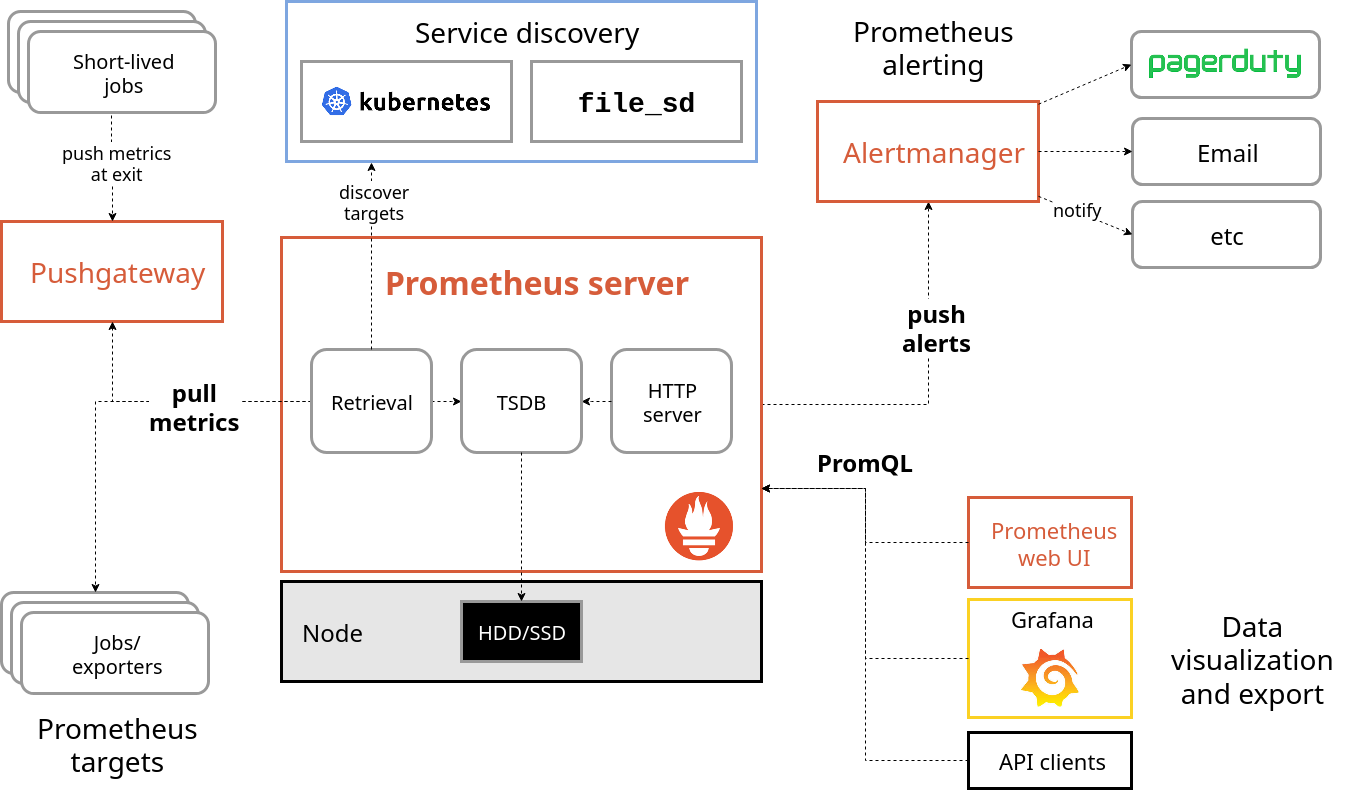
\includegraphics[width=\linewidth, keepaspectratio]{./figures/prometheus_arch}
    \caption{Prometheus Architecture}
\end{figure}

Prometheus fundamentally stores all data as \textit{time series}: streams of timestamped
values belonging to the same metric and the same set of labeled dimensions~\cite{prometheus_data_model}.\\

Time series are uniquely identified by their metric name and optional key-value pairs called labels.\\
The names of time series must comply with the following rules:

\begin{itemize}
    \item \textbf{SHOULD} specify the general feature of a system that is measured.
    \item \textbf{MAY} use any UTF-8 characters.
    \item \textbf{SHOULD} match the regex \texttt{[a-zA-Z\_:][a-zA-Z0-9\_:]*} for the best experience and
    compatibility.
    Metric names outside of that set will require quoting.
\end{itemize}

Metric labels must comply with the following rules:

\begin{itemize}
    \item Both names and values \textbf{MAY} use any UTF-8 characters.
    \item If the name of a metric begins with two underscores, said metric \textbf{MUST} be reserved for internal
    Prometheus use.
    \item \textbf{SHOULD} match the regex \texttt{[a-zA-Z\_:][a-zA-Z0-9\_:]*} for the best experience and
    compatibility.
    Metric names outside of that set will require quoting.
    \item Labels with an empty label value are considered equivalent to labels that do not exist.
\end{itemize}


\medskip
\noindent
\textbf{NOTE:} Colons (\texttt{:}) in for both label and metric names regex are reserved for user-defined recording
rules.
They \textbf{SHOULD NOT} be used by exporters or direct instrumentation.

Time series are identified using the following notation:
\begin{figure}[h]
    \centering
    \begin{lstlisting}
<metric name>{<labelN name>="<labelN value>", ...}
    \end{lstlisting}
    \caption{Example of a distributed trace log}
\end{figure}

Samples form the actual time series data, they are the most basic unit of data in Prometheus.
Each sample consists of a float64 or native histogram value, and a millisecond-precision timestamp.\\

\subsection{Metric Types}\label{subsec:metric-types}

Prometheus client libraries offer four core metric types, as of the time of writing of this report the Prometheus
server does not make use of the type information of these metrics and all data is flattened to untyped time series.
Only client libraries, to enable \ac{API}s tailored to the usage of specific types and the wire protocol make use of
type information of the metrics~\cite{prometheus_metric_types}.\\

\textbf{Counter} - A counter represents a cumulative metric that a value whose value can only change upwards with
the ability of being reset to zero on restart.
An example use case would be counting the number of requests made to an \ac{API}.\\

\textbf{Gauge} - A gauge is a metric that represents a value that can change either upwards or downwards, typically
used for measured values like temperatures, disk utilization or, for example, the number of active connections
to a database at a given moment.

\textbf{Histogram} – A histogram samples observations (usually things like request durations or response sizes) and counts them in configurable buckets.
It provides a way to understand the distribution of values by showing how many observations fall into each bucket.
Histograms also automatically calculate the sum and count of all observed values, enabling the computation of averages and percentiles.

\textbf{Summary} – A summary also samples observations and provides a total count, sum, and configurable quantiles (percentiles) over a sliding time window.
Unlike histograms, summaries calculate quantiles on the client side, making them useful for tracking latency distributions or other metrics where precise quantiles are needed.
However, summaries are not aggregated across multiple instances as easily as histograms.


\section{Existing Prometheus Clients}\label{sec:existing-prometheus-clients}

Prometheus supports a variety of official client libraries that enable instrumenting applications to expose
metrics in a format compatible with the Prometheus server.
These official clients cover popular programming languages such as Go, Java, Python, Ruby, and Rust.
Additionally, the Prometheus community encourages developers to create and maintain client libraries for languages not yet officially supported, fostering a diverse ecosystem of instrumentation tools.

The official client libraries include:
\begin{itemize}
    \item \texttt{client\_golang} for Go
    \item \texttt{client\_java} for Java and \ac{JVM} languages
    \item \texttt{client\_python} for Python
    \item \texttt{client\_ruby} for Ruby
    \item \texttt{client\_rust} for Rust
\end{itemize}

Some notable unofficial (community-driven) client libraries include:
\begin{itemize}
    \item \texttt{prometheus-client-c} for C
    \item \texttt{prometheus-cpp} for C++
    \item \texttt{prometheus-net} for .NET/C\#
    \item \texttt{prom-client} for Node.js
    \item \texttt{prometheus\_client\_php} for PHP
\end{itemize}

This ongoing effort helps ensure Prometheus instrumentation can be integrated across a wide range of applications and environments.

\section{The Kotlin Ecosystem and Observability Gaps}\label{sec:the-kotlin-ecosystem-and-observability-gaps}

While the official Prometheus Java client library is widely used across the \ac{JVM} ecosystem, it is primarily
designed with Java’s language features and idioms in mind.
This design choice limits its ability to fully leverage Kotlin-specific features such as coroutines, extension functions, and null safety.
Consequently, using the Java client directly in Kotlin projects can lead to suboptimal performance and non-idiomatic code patterns.

For example, popular Kotlin frameworks like \texttt{Ktor} currently lack out-of-the-box support from the official Prometheus client.
This gap forces developers to write custom wrappers or adapters, increasing both development complexity and maintenance overhead.
Additionally, the Java client does not always seamlessly integrate with Kotlin’s coroutine-based concurrency model, which can hinder efficient metric instrumentation.

Recognizing these challenges, the Prometheus project encourages the development of language-specific client libraries.
It provides clear guidelines on best practices and pitfalls to avoid when creating such libraries, helping ensure consistency and quality across implementations.
Moreover, Prometheus maintains an active mailing list where developers can seek clarification and feedback directly from core Prometheus maintainers.
This open line of communication supports community-driven efforts to fill observability gaps in ecosystems like Kotlin, fostering better integration and more idiomatic instrumentation libraries.
